\documentclass[12pt,a4paper]{report}
\usepackage[utf8]{inputenc}
\usepackage[T1]{fontenc}
\usepackage[spanish]{babel}
\usepackage{amsmath}
\usepackage{amsfonts}
\usepackage{amssymb}
\usepackage{graphicx}
\usepackage[left=1.5cm,right=1.5cm,top=1.5cm,bottom=1.5cm]{geometry}
\usepackage{listings}

\lstset
{
    language=C,
  	breaklines=true
    basicstyle=\ttfamily,
    keywordstyle=\bfseries,
    showstringspaces=false
}

\title{\Huge Informe sobre el Proyecto de Programación Moogle!}
\author{Lianny de la Caridad Revé Valdivieso \\ Facultad de Matemática y Computación \\ Universidad de La Habana}
\date{\today}

\begin{document}

\maketitle

\chapter*{Introducción}

\begin{figure}[h]
    \centering
    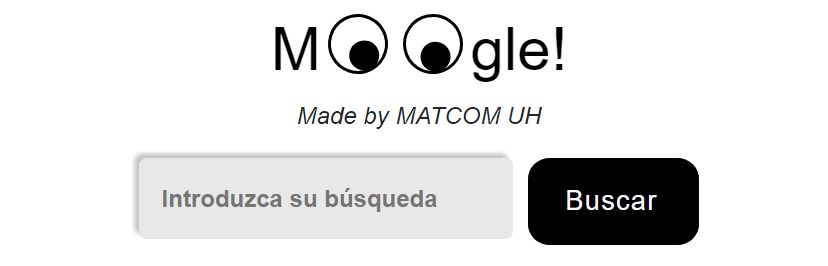
\includegraphics[height=5cm]{MoogleSearcher}
\end{figure}

\vspace{1cm}

\textbf{Moogle!} es una aplicación cuyo propósito es buscar inteligentemente un texto en un conjunto de documentos.
Es una aplicación web, desarrollada con tecnología.NET Core 7.0, específicamente usando Blazor como framework web para la interfaz gráfica, y en el lenguaje C\#. La aplicación está dividida en dos componentes fundamentales:
\begin{itemize}
	\item \texttt{MoogleServer} es un servidor web que renderiza la interfaz gráfica y sirve los resultados.
	\item \texttt{MoogleEngine} es una biblioteca de clases donde está implementada la lógica del algoritmo de búsqueda.
\end{itemize}
Al iniciar el servidor, este crea una instancia de Motor de Búsqueda, el cual carga los documentos y los procesa individualmente para obtener los datos relevantes sobre ellos, tales como su nombre, ruta y frecuencia de sus términos, estos luegos son utilizados para crear un Diccionario que contiene todos los términos del corpus textual(los documentos), con esto se calcula por cada término de cada documento su frecuencia inversa o IDF y se utiliza esta métrica para normalizar la frecuencia del término en el documento o TF, y así definir la relevancia de cada uno de los documentos, y en el Diccionario estos valores son almacenados para utilizarse en las búsquedas.\par
Cuando el usuario realiza una consulta mediante la interfaz gráfica esta pasa al servidor, donde se procesan los datos introducidos por el usuario tales como: separar y procesar los términos y calcular a cada uno de ellos su relevancia de la misma manera que se efectuó con los documentos del corpus. Tras desarrollarlo, se procede a reducir el espacio de búsqueda mediante el cálculo de la puntuación o score de cada documento respecto a la query, esto se cubre utilizando la distancia coseno entre vectores, luego de calcular todos los scores, se organiza la lista de documentos según su score de mayor a menor y se devuelven al usuario.\par
En caso de que el directorio que contiene los documentos esté vacío, no se introduzca ninguna consulta, o hubo alguna palabra que no se pudo encontrar no será devuelto ningún resultado y el usuario deberá realizar una nueva búsqueda.\par
Para implementar el algoritmo de búsqueda, hemos creado e implementado varias clases fundamentales. Cada clase es una abstracción de los componentes del motor de búsqueda. A continuación las abordaremos a detalle.


\chapter*{Clase DataFile}
\texttt{DataFile} es una clase creada como abstracción de lo que representa un documento en nuestro motor de búsqueda.

\begin{lstlisting}
public string FileRoot {get; private set;} // ruta del archivo

public string FileName {get; private set;} // nombre del archivo

public string FileContent {get; private set;} // contenido del archivo sin procesar

public int FileWords {get; private set;} // cantidad de palabras por archivo

public string[] AllWordsOnFile {get; set;} // array que contiene todas las palabras del archivo

public Dictionary <string, float> WordFreq {get; set;} // diccionario que contiene el conjunto de palabras de un documento y su TF
\end{lstlisting}

Hemos declarado cada una de las propiedades públicas ya que necesitaremos acceder a ellas fuera desde otras clases. \par\bigskip
El objeto \texttt{DataFile} recibe en su construcctor un argumento de tipo string \texttt{root}, que vendría siendo la ruta del documento (también denominado path) dentro del directorio de documentos.

\begin{lstlisting}
public DataFile(string root)
       	{   
            FileRoot = root;

            FileName = GetFileName(root); 

            FileContent = GetFileContent(root); 
           
            AllWordsOnFile = Tools.TxtProcesser(FileContent);

            FileWords = AllWordsOnFile.Length; 

            WordFreq = TFCalculator(AllWordsOnFile);
        }
\end{lstlisting}

A la propiedad \texttt{FileRoot} se le asigna el mismo string recibido en el constructor (el path del archivo), y la propiedad \texttt{AllWordsOnFile} utiliza un método perteneciente a la clase \texttt{Tools} (ver Clase Tools). El resto de las propiedades utilizan los métodos que veremos a continuación.\par\bigskip

El método \texttt{GetFileName()} recibe como parámetro la ruta del documento recibida en el constructor de la clase y devuelve un string con el nombre del documento.Es un método privado ya que solo será utilizado dentro del campo de la clase DataFile. Para obtener el nombre del archivo utiliza dos métodos pertenecientes a la clase \texttt{Path} (System.IO como namespace)
\begin{itemize}
\item \texttt{GetFileName()} que recibe como parámetro un string que es la ruta del documento, y devuelve el nombre del archivo y la extensión del mismo.
\item \texttt{ChangeExtension()} que recibe como parámetros un string con la información de la ruta a modificar, y otro string con la nueva extensión, en nuestro caso especificamos \texttt{null} para eliminar la extensión y quedarnos solo con el nombre del documento.
\end{itemize}

\begin{lstlisting}

        private static string GetFileName(string root)
        {
            string FileName = Path.GetFileName(root); // obtenemos el nombre del archivo con su extension
            FileName = Path.ChangeExtension(FileName, null); // anulamos la extension
            
            return FileName;
        }

\end{lstlisting}\bigskip

El método \texttt{GetFileContent()} recibe como parámetro la ruta del documento recibida en el constructor de la clase y devuelve un string con el contenido del documento sin tokenizar.Es un método privado ya que solo será utilizado dentro del campo de la clase DataFile. Para obtener el contenido del archivo utiliza un método a través de una instancia de la clase \texttt{StreamReader} (System.IO como namespace).\par
El método \texttt{ReadToEnd()} lee todos los caracteres desde la primera posición del string hasta el final del mismo.

\begin{lstlisting}
        private static string GetFileContent(string root)
        {
            StreamReader reader = new StreamReader(root); // leemos el contenido del archivo
            string FileContent = reader.ReadToEnd();
            reader.Close(); 

            return FileContent;
        }
\end{lstlisting}\bigskip

El método \texttt{TFCalculator()} recibe como parámetro el array que contiene cada palabra del documento tokenizada, y devuelve un Diccionario que contiene como llave cada palabra de un documento sin repetirse, y como valor el TF de cada palabra en el documento.\par
TF singnifica Term Frequency o Frecuencia del término en español, y es la cantidad de veces que un término aparece en un documento dado, dividido por el número total de de palabras de un documento. 
Ya que el TF de un término está ligado a un documento en específico, el cálculo del TF es un método privado perteneciente a la clase DataFile y tendremos un diccionario de este tipo por cada documento en nuestro directorio de documentos.\par 

\begin{lstlisting}
private static Dictionary<string, float> TFCalculator(string[] AllWordsOnFile)
        {   
            Dictionary<string, float> WordFreq = new Dictionary<string, float>();
            float maxFreq = 0;
            foreach(string word in AllWordsOnFile)
                {  
                    if(!WordFreq.Keys.Contains(word)) // si la palabra no estaba en el documento la cargamos y aparece 1 vez
                    {
                        WordFreq.Add(word, 1);
                    }
                    else // si la palabra ya estaba en el documento aumentamos su valor en 1
                    {
                        WordFreq[word]++;
                        maxFreq = Math.Max(maxFreq , WordFreq[word]);
                    }
                }

                foreach(string key in WordFreq.Keys)
                {
                    WordFreq[key] = WordFreq[key]/maxFreq; // tomamos el TF de un termino en un documento como el numero de apariciones del termino en un documento / numero total de palabras del documento
                }

            return WordFreq;
        }
\end{lstlisting}\par\bigskip

El siguiente fragmento de código contiene tres métodos \texttt{FragmentWithWords()}, \texttt{Partition()} y \texttt{WordsImportant()}.\par

El método llamado FragmentWithWords(), es el principal, que toma como parámetros un array de string llamado query(que contiene cada palabra de la query tokenizada), una cadena llamada root(el path del documento) y un diccionario llamado IDF(que contiene todas las palabras del corpus textual como llaves, y como valores, el IDF correspondiente a cada una (ver clase DataFolder)). El método devuelve una cadena que representa un fragmento de texto denominado snippet.\par

El método comienza leyendo el contenido de un archivo cuya ruta se especifica en el parámetro root. Luego, el contenido del archivo se transforma a minúsculas y se aplica una transformación utilizando el método \texttt{Tools.Transform()} (ver clase Tools). Después, el contenido se divide en palabras utilizando el método Split() con un espacio como separador y se eliminan las entradas vacías.\par

El método continúa extrayendo las palabras importantes de la consulta utilizando el método \texttt{WordsImportant()}, que toma como parámetros el array de string query y el diccionario IDF. Este método devuelve un arreglo de cadenas que contiene las palabras importantes de la consulta.Para determinar que una palabra tiene importancia se verifican tres condiciones: la palabra debe existir en el corpus textual, el IDF de la palabra debe ser distinto de cero, la palabra debe tener más de tres letras (así eliminamos los artículos, la mayoría de las perposiciones y otras palabras sin relevancia).

Luego, el método entra en un bucle while que se ejecuta mientras la longitud del array de string sea mayor que 80. Dentro del bucle, el arreglo de palabras se divide en dos partes utilizando el método texttt{Partition()}. Luego, se comparan las dos partes para ver cuál contiene más palabras importantes de la consulta. La parte que contiene más palabras importantes se guarda en el array de palabras y el proceso se repite hasta que la longitud del array de palabras sea menor o igual a 80.

Finalmente, el método genera el resultado concatenando las palabras del array de palabras. Si una palabra es importante (está contenida en el array de palabras importantes), se agrega al resultado rodeada por asteriscos para resaltarla. El resultado final se devuelve rodeado por puntos suspensivos.

\begin{lstlisting}
        public string FragmentWithWords(string[] query, string root, Dictionary <string, float> IDF)
        {
            StreamReader reader = new StreamReader(root);
            string content = reader.ReadToEnd().ToLower();
            reader.Close();
            content = Tools.Transform(content);

            string[] words = content.Split(' ', StringSplitOptions.RemoveEmptyEntries);

            int part1 = 0; // contadores para comparar
            int part2 = 0;

            string[] Query = WordsImportant(query, IDF); // extraemos las palabras que tienen relevancia en la query

            while (words.Length > 80) // solo devolveremos un maximo de 80 palabras
            {
                // partimos a la mitad el array
                string[] Part1 = Partition(words, 0, words.Length / 2);
                string[] Part2 = Partition(words, words.Length / 2, words.Length);

                int count = 0;

                for (int i = 0; i < Math.Min(Part1.Length, Part2.Length); i++)
                {
                    count++;
                    if (Query.Contains(Part1[i]))
                    { 
                        part1++; // aumentamos en una unidad el valor del comparador
                    }
                    if (Query.Contains(Part2[i]))
                    {
                        part2++; // aumnetamos en una unidad el valor del comparador
                    }
                }
                if (Part1.Length > Part2.Length)
                {
                    for (int i = count; i < Part1.Length; i++)
                    {
                        if (Query.Contains(Part1[i]))
                        {
                            part1++;
                        }
                    }
                }
                if (Part2.Length > Part1.Length)
                {
                    for (int i = count; i < Part2.Length; i++)
                    {
                        if (Query.Contains(Part2[i]))
                        {
                            part2++;
                        }
                    }
                }
                if (part1 >= part2) // nos quedamos con la que mas resultados tuvo
                    words = Part1;
                else
                    words = Part2;
                part1 = 0;
                part2 = 0;
            }

            string result = "";

            foreach (string a in words) // generamos el texto a devolver
            {
                if (Query.Contains(a))
                    result += "**" + a + "** ";
                else
                    result += a + " ";
            }

            return "........" + result + "........";
        } 

        string[] Partition(string[]words,int stratindex,int endindex)
        {
            string[] result = new string[endindex - stratindex];
            int position = 0;
            for(int i = stratindex; i < endindex; i++)
            {
                result[position] = words[i];
                position++;
            }
            return result;
        }
        string[] WordsImportant(string[] AllWordsOnFile, Dictionary <string, float> IDF)
        {
            List<string> result = new List<string>();

            foreach(string word in AllWordsOnFile)
            {   
                if(IDF.ContainsKey(word) && IDF[word] != 0 && word.Length > 3)
                result.Add(word);
            }

            return result.ToArray();
        }

\end{lstlisting}

\chapter*{Clase DataFolder}

\texttt{DataFolder} representa un directorio o contenedor de documentos (o DataFiles), con sus propiedades y métodos propios.Como propiedades de la clase encontramos las siguientes:

\begin{lstlisting}
        public string[] FilesRoot {get; set;} // array para guardar las rutas de los archivos
        public DataFile[] Files {get; set;} // array de objetos tipo DataFile
        public int NumberOfFiles {get; private set;} // cantidad de archivos a nivel de carpeta
        public Dictionary <string, Dictionary <string, float>> TF; // diccionario que contiene los TF de cada termino por cada documento
        public Dictionary <string, Dictionary <string, float>> Relevance; // diccionario que contiene la relevancia de cada palabra por cada documento 
        public static Dictionary <string, float> IDF {get; set;} // diccionario que contiene cada palabra del corpus textual con su IDF
\end{lstlisting}\bigskip

Hemos declarado cada una de las propiedades públicas ya que necesitaremos acceder a ellas fuera desde otras clases.\par\bigskip
El objeto \texttt{DataFolder} recibe en su constructor un argumento de tipo string \texttt{root}, que vendría siendo el path de la carpeta de documentos llamada Content.

\begin{lstlisting}
        public DataFolder(string root)
        {   
            //instanciamos los diccionarios
            TF = new Dictionary<string, Dictionary<string,float>>(); 
            Relevance = new Dictionary<string, Dictionary<string,float>>();
            IDF = new Dictionary<string, float>();

            FilesRoot = Directory.EnumerateFiles(root, "*.txt").ToArray(); // obtenemos las rutas de todos los archivos de la carpeta
            
            NumberOfFiles = FilesRoot.Length;

            Files = new DataFile[NumberOfFiles];

            Console.WriteLine("Cargando archivos...");

            int count = 0;

            foreach(string path in FilesRoot) // por cada ruta en el array de rutas
            {
                DataFile file = new DataFile(path); // creamos un objeto de tipo DataFile
                Files[count] = file;
                count++;

                System.Console.WriteLine($"Cargando archivo {file.FileName}");

                TF.Add(file.FileName, file.WordFreq); // agregamos la frecuencia de cada palabra en cada archivo al diccionario de TFs
                Relevance.Add(file.FileName, file.WordFreq); // agregamos la frecuencia de cada palabra en cada archivo al diccionario de Relevancias para modificar despues su valor
            }

            foreach(DataFile file in Files) // objeto de tipo DataFile en el array de DataFiles
            {
                foreach(string word in file.WordFreq.Keys) // por cada palabra del DataFile
                {
                    if(!IDF.ContainsKey(word)) // si la palabra no esta contenida en el diccionario de los IDFs
                    IDF.Add(word, idfCalculator(word)); // la agregamos al diccionario y calculamos su IDF

                    Relevance[file.FileName][word] = relevanceCalculator(file.FileName, word); // calculamos el valor de la relevancia para cada palabra de cada archivo en el diccionario de las relevancias
                }
            }

            System.Console.WriteLine($"Han sido cargados {NumberOfFiles} archivos");

        }

\end{lstlisting}

Nuestro constructor realiza las siguientes acciones:
\begin{itemize}
\item Instancia los diccionarios \texttt{TF}, \texttt{Relevance} e \texttt{IDF}.

\item Obtiene las rutas de todos los archivos de texto en la carpeta especificada por \texttt{root} y las guarda en el array \texttt{FilesRoot}. La propiedad \texttt{FilesRoot} utiliza el método \texttt{EnumerateFiles()} de la clase \texttt{Directory} (System.IO como namespace). Este método recibe como parámetro un string que representa la ruta del directorio de los documentos, y devuelve una colección enumerable de rutas que coinciden con la extensión ".txt".

\item Establece el valor de la propiedad \texttt{NumberOfFiles} como la longitud del array \texttt{FilesRoot}, a través de la propiedad \texttt{Length}.

\item Crea un array de objetos \texttt{DataFile} con una longitud igual a \texttt{NumberOfFiles}.

\item Recorre cada ruta en el array \texttt{FilesRoot}, crea un objeto \texttt{DataFile} para cada ruta y lo agrega al array \text{Files}.

\item Agrega la frecuencia de cada palabra en cada archivo al diccionario de TFs y al diccionario de Relevancias.

\item Recorre cada objeto \texttt{DataFile} en el array \texttt{Files} y, para cada palabra del archivo, verifica si está contenida en el diccionario de IDFs. Si no está contenida, agrega la palabra al diccionario y calcula su IDF.

\item Calcula el valor de la relevancia para cada palabra de cada archivo en el diccionario de las relevancias a través del método \texttt{idfCalculator()} que veremos a continuación.

\end{itemize}\bigskip

El siguiente fragmento de código contiene dos métodos: el método principal \texttt{idfCalculator()} y su método auxiliar \texttt{countContains()}. Nuestro método principal recibe como parámetro un string palabra, y devuelve su IDF.\par
El IDF de una palabra significa Inverse Document Frequency o Frecuencia inversa de documento en español, y se calcula con la siguiente fórmula:\par

$$IDF(t) = log(\frac{N}{DF(t)})$$ \bigskip

donde \textbf{N} es la cantidad total de documentos y \textbf{DF(t)} la cantidad de documentos en los que aparece \textbf{t} (el término). en caso de que un término no aparezca en ningún documento, el valor del IDF es cero. El método \texttt{countContains()} calcula el valor de \textbf{DF(t)}.\par

\begin{lstlisting}
        private int countContains(string word) // metodo que cuenta en cuantos documentos esta contenida una palabra
        {
            int count = 0;
            foreach (string doc in TF.Keys)
            {
                if (TF[doc].ContainsKey(word)) // si la palabra esta contenida en el diccionario
                {
                    count++; // aumenta una unidad la cantidad de veces que aparece la palabra
                }
            }
            return count;
        }

        private float idfCalculator(string word) // metodo que calcula el tf de una palabra (log natural de la razon entre el numero total de archivos y el numero de archivos que contienen dicha palabra (formula smooth))
        {
            float IDF = (float)Math.Log10((float)NumberOfFiles / ((float)countContains(word) +1)) +1;
            return IDF;
        }
\end{lstlisting}\bigskip

Por último, el método \texttt{relevance calculator} calcula la relevancia de un documento en relación a una palabra específica utilizando los valores de frecuencia de término (TF) e inversa de frecuencia de documento (IDF). La relevancia está dada por la multiplicación de estos dos valores

\begin{lstlisting}
        private float relevanceCalculator(string document, string word) // metodo que calcula la relevancia de un documento en relacion a una palabra
        {
            float tf = TF[document][word];
            float idf = idfCalculator(word);

            float relevance = tf * idf;

            return relevance;
        }
\end{lstlisting}

\chapter*{Clase Query}

\texttt{Query} es la clase que representa y procesa la consulta realizada por el usuario. Contiene las siguientes propiedades:\par
\begin{lstlisting}
        public string InputQuery {get; set;} // string introducido por el usuario
        public Dictionary <string, float> DataQuery; // diccionario que almacena la relevancia de cada palabra de la query
        public string[] QueryWordsArray {get; private set;} // array que las palabras de la query
\end{lstlisting}\bigskip

El objeto \texttt{Query} recibe en su constructor un argumento de tipo string \texttt{input} que vendría siendo la consulta introducida por el usuario mediante la interfaz gráfica.\par

\begin{lstlisting}
        public Query(string input)
        {
            InputQuery = input;

            QueryWordsArray = Tools.TxtProcesser(InputQuery); // procesamos la query

            DataQuery = GetQueryRelevance(QueryWordsArray); // obtenemos el diccionario con la relevancia
        
            System.Console.WriteLine($"La Query {input} ha sido cargada");
        }

\end{lstlisting}\bigskip

El valor de la propiedad \texttt{InputQuery} se establece a través del parámetro recibido en el constructor.\par
La propiedad \texttt{QueryWordsArray} utiliza el método \texttt{Tools.TxtProcesser()} (ver clase Tools).\par
La propiedad \texttt{DataQuery} utiliza el método \texttt{GetQueryRelevance()} que veremos a continuación.\par\bigskip

El método \texttt{GetQueryRelevance()} recibe como parámetro un array de string donde se encuentran cada palabra de la query tokenizada, y devuelve un diccionario que tiene como llave cada palabra de la query y como valor su relevancia.
El método recorre el array de palabras de la query y obtiene de forma individual su TF e IDF. Luego los multiplica para obtener la relevancia.\par 

\begin{lstlisting}
        static private Dictionary <string, float> GetQueryRelevance(string[] QueryWordsArray) // array que devuelve un diccionario que tiene como llave cada palabra de la query, y como value su relevancia
        {   
            Dictionary <string, float> DataQuery = new Dictionary <string, float>();

            foreach(string word in QueryWordsArray) // por cada palabra en la query
            {
                if(!DataQuery.Keys.Contains(word)) // si el diccionario no contenia la palabra
                DataQuery.Add(word, 1); // la anadimos y le asignamos una frecuencia de 1
 
                else // si la palabra ya se encontraba en el diccionario
                DataQuery[word]++; //aumentamos su frecuencia en 1
            }

            foreach(string key in DataQuery.Keys)
            {
                DataQuery[key] = DataQuery[key]/QueryWordsArray.Length;; // calculamos el TF de la query
                if(DataFolder.IDF.ContainsKey(key))
                {
                    DataQuery[key] = DataQuery[key] * DataFolder.IDF[key];
                } // multiplicamos el TF*IDF para obtener la relevancia de cada palabra de la query
            }

            return DataQuery;
        }
\end{lstlisting}

\chapter*{Clase Tools}

La clase \texttt{Tools} contiene las herramientas (métodos) para procesar texto. Está compuesta por dos métodos principales y un método auxiliar.\par\bigskip

\texttt{TxtProcesser()} es un método principal público que toma un string como entrada y devuelve un array de palabras normalizadas. El método primero convierte el string de entrada en minúsculas utilizando el método \texttt{ToLower()}. Luego, llama al método \texttt{RemoveAccentsAndPuntuations()} para eliminar todos los signos de puntuación de la cadena de entrada. Finalmente, el método divide el string de entrada en palabras utilizando el método \texttt{Split()} con espacio como separador y \texttt{StringSplitOptions.RemoveEmptyEntries} como opción para eliminar cualquier entrada vacía del array resultante.

\texttt{RemoveAccentsAndPuntuations} es un método auxiliar privado que toma un string como entrada y devuelve una nuevo string con todos los signos de puntuación eliminados. El método utiliza el método \texttt{Regex.Replace} para reemplazar todos los caracteres que no son letras, números o espacios con un carácter de espacio. El string de entrada se normaliza primero utilizando el método \texttt{Normalize} con el parámetro \texttt{NormalizationForm.FormD}.

\begin{lstlisting}
    private static string RemoveAccentsAndPuntuations(string inputString) // metodo que elimina todos los signos de puntuacion
    {
        return Regex.Replace(inputString.Normalize(NormalizationForm.FormD), @"[^a-zA-z0-9 ]+", " "); 
    }

    public static string[] TxtProcesser(string inputString) // metodo que procesa el contenido de un archivo y devuelve un array de palabras normalizadas
    {
        inputString = inputString.ToLower(); // llevamos todo el contenido a minusculas
        inputString = RemoveAccentsAndPuntuations(inputString); // removemos todos los signos de puntuacion
        string[] words = inputString.Split(' ', StringSplitOptions.RemoveEmptyEntries); // dividimos en palabras y guardamos en un array

        return words;
    }

\end{lstlisting}\bigskip

El siguiente es un método principal llamado \texttt{Transform()} que toma un parámetro de tipo \texttt{string} llamado \texttt{value}. El propósito de este método es eliminar ciertos caracteres innecesarios al leer un archivo de texto. 

El método define un array de caracteres llamada \texttt{guide} que contiene los caracteres que se deben eliminar: \texttt{\textbackslash r}, \texttt{\textbackslash n}, \texttt{(}, \texttt{)}, \texttt{*}, \texttt{\{}, \texttt{\}}, \texttt{´}, \texttt{\`}, \texttt{,}, \texttt{.}, y \texttt{:}. Luego, el método utiliza un bucle \texttt{foreach} para iterar sobre cada uno de estos caracteres en el array \texttt{guide}. Dentro del bucle, el método utiliza el método \texttt{Replace()} para reemplazar todas las ocurrencias del carácter actual en el string \texttt{value} con un espacio en blanco. Finalmente, el método devuelve el string modificado \texttt{value} modificada.

\begin{lstlisting}
    public static string Transform(string value)//metodo que elimina los caracteres innecesarios al leer un txt
    {
        char[] guide = { '\r', '\n', '(', ')', '*', '{', '}', '`' ,',','.',':'}
        foreach (char a in guide)
        {
            value = value.Replace(a, ' ');
        }
        return value;
    }
\end{lstlisting}

\chapter*{Clase Engine}

La clase \texttt{Engine} es la clase que se encarga de manejar los objetos de tipo \texttt{DataFile}, \texttt{DataFolder} y \texttt{Query} para la obtención de objetos tipo \texttt{SearchItem} y posteriormente de tipo \texttt{SearchResult} que son los devueltos al usuario.
La clase consta de un método principal \texttt{Query()} y dos métodos auxiliares: \texttt{ScoreCalculator()} y \texttt{Sort()}.

El método \texttt{ScoreCalculator()} calcula el puntaje de un documento utilizando el modelo vectorial de distancia coseno.\par

El modelo vectorial de distancia coseno es una medida de similitud entre dos vectores no nulos definidos en un espacio de producto interno. La similitud coseno es el coseno del ángulo entre los vectores; es decir, es el producto escalar de los vectores dividido por el producto de sus longitudes.\par

En el contexto de la recuperación de información y la minería de texto, cada palabra se asigna a una coordenada diferente y un documento se representa mediante el vector de los números de ocurrencias de cada palabra en el documento. La similitud coseno proporciona entonces una medida útil de cuán similares son dos documentos en términos de su contenido, independientemente de la longitud de los documentos.\par

El método toma tres argumentos: \texttt{ToSearch}, que es una consulta de búsqueda; \texttt{Docs}, que es un diccionario que contiene los documentos y sus respectivas palabras con sus pesos; y \texttt{file}, que es el nombre del archivo para el cual se calculará el puntaje.\par

El método comienza inicializando tres variables: \texttt{dotProduct}, \texttt{dim1} y \texttt{dim2}. Luego, itera sobre todas las palabras en el documento especificado por el argumento \texttt{file}. Si la palabra no está presente en la consulta de búsqueda, se agrega 0 al producto punto. De lo contrario, se agrega el producto de los pesos de la palabra en la consulta y el documento al producto punto. Además, se calcula la norma del vector 2 (la consulta) sumando el cuadrado del peso de la palabra en la consulta.\par

Después de iterar sobre todas las palabras en el documento, se calcula la norma del vector 1 (el documento) sumando el cuadrado del peso de cada palabra en el documento. Finalmente, se devuelve el cociente del producto punto y el producto de las raíces cuadradas de las normas de los vectores 1 y 2. Esto es equivalente a calcular la distancia coseno entre los dos vectores.\par

\begin{lstlisting}
        private static float ScoreCalculator (Query ToSearch, Dictionary < string, Dictionary<string, float>> Docs, string file) // metodo que calcula el score
        {
            float dotProduct = 0;
            float dim1 = 0;
            float dim2 = 0;

            foreach(string word in Docs[file].Keys)
                {
                    if(!ToSearch.DataQuery.ContainsKey(word))
                        dotProduct += 0;
                    else
                    {
                        dotProduct += ToSearch.DataQuery[word] * Docs[file][word];  
                        dim2 += (float)Math.Pow(ToSearch.DataQuery[word], 2); //para calcular la norma del vector 2
                    }

                    dim1 += (float)Math.Pow(Docs[file][word], 2); // para calcular la norma del vector 1
                }
            return dotProduct / ((dim1==0 || dim2==0)?1:(float)(Math.Sqrt(dim1) * Math.Sqrt(dim2))); // distancia coseno 
        }
\end{lstlisting}\bigskip

El método \texttt{Sort()} recibe como parámetro un array de \texttt{SearchItem} y los ordena según sus scores de mayor a menor. Luego devuelve el array ordenado.\par

\begin{lstlisting}
        private static SearchItem[] Sort(SearchItem[] docs_score)// metodo que ordena el array de SearchItem segun sus scores
        {
            for (int i = 0; i < docs_score.Length; i++)
            {
                for (int j = i; j < docs_score.Length; j++)
                {    if (docs_score[j].Score > docs_score[i].Score)
                    {
                        SearchItem temp = docs_score[j];
                        docs_score[j] = docs_score[i];
                        docs_score[i] = temp;
                    }
                }
            }

            return docs_score;
        }    

\end{lstlisting}\bigskip


El método \texttt{Query} es una función de búsqueda que recibe una consulta (\texttt{query}) y un contenedor de archivos (\texttt{Content}) y devuelve el resultado de la búsqueda en forma de un objeto \texttt{SearchResult}. 

El método comienza asignando la consulta a una variable llamada \texttt{suggestion} y creando un objeto \texttt{Query} con la consulta. Luego, se crea un diccionario llamado \texttt{Docs} que contiene la relevancia de los documentos en el contenedor de archivos.

Se crea una lista llamada \texttt{docs\_Scores} para almacenar objetos de tipo \texttt{SearchItem}. Luego, para cada archivo en el contenedor, se obtiene su título, un fragmento del archivo que contiene las palabras de la consulta (llamado \texttt{snippet}) y un puntaje calculado por la función \texttt{ScoreCalculator}. Con esta información, se crea un objeto \texttt{SearchItem} y, si su puntaje y su snippet no son nulos, se agrega a la lista \texttt{docs\_Scores}.\par

Después, se crea un arreglo llamado \texttt{Items} con una longitud de 20 para almacenar los resultados de la búsqueda. Se ordena la lista \texttt{docs\_Scores} y se llena el arreglo \texttt{Items} con los primeros 20 elementos de la lista ordenada.\par

Finalmente, se muestra un mensaje indicando que los resultados han sido devueltos y se muestra el título y el puntaje de cada elemento en el arreglo \texttt{Items}. El método devuelve un nuevo objeto \texttt{SearchResult} creado con el arreglo \texttt{Items} y la variable \texttt{suggestion}.par\

\begin{lstlisting}
        public static SearchResult Query(string query, DataFolder Content) // metodo que recibe una query y un contenedor de archivos y devuelve el resultado de la busqueda
        {   
            string suggestion = query; // asiganamos a la sugerencia el mismo string que la query 
            Query ToSearch = new Query(query); // creamos con la query un objeto de tipo Query

            Dictionary < string, Dictionary<string, float>> Docs = Content.Relevance;

            List<SearchItem> docs_Scores = new List<SearchItem>(); // creamos una lista para guardar los objetos de tipo SearchItem
            
            foreach(DataFile file in Content.Files) // por cada archivo en el contenedor
            {
                string tittle = file.FileName; // obtenemos su titulo
                string snippet = file.FragmentWithWords(ToSearch.QueryWordsArray, file.FileRoot, DataFolder.IDF); // obtenemos su snippet
                float score = ScoreCalculator(ToSearch, Docs, file.FileName); // obtenemos su score

                SearchItem item = new SearchItem(tittle, snippet, score); // creamos un objeto de tipo SearchItem

                if(item.Score != null && item.Snippet != null) // si el score o el snippet son distintos de null
                {
                    docs_Scores.Add(item); // anadimos el objeto a la lista 
                }
            }
    	    
            SearchItem[] Items = new SearchItem[20]; // creamos el array para devolver con 20 resultados

            SearchItem[] sortedScores = Sort(docs_Scores.ToArray()); // ordenamos la lista de SearchItem llevado a array 

            for(int i = 0; i < Items.Length; i++)
            {
            Items[i] = sortedScores[i]; // llenamos el array a devolver con los primeros SearchItem del array de SearchItem ordenado
            }
            

            System.Console.WriteLine("Los resultados han sido devueltos");

            foreach(SearchItem item in Items)
            {
                System.Console.WriteLine($"el item {item.Title} tiene un score de {item.Score}");
            }

            return new SearchResult(Items, suggestion);
        }

\end{lstlisting}

\chapter*{Clase Moogle}

Finalmente, la clase Moogle es la clase a la que accede el servidor web a la hora de realizar la búsqueda. La clase consta de dos propiedades (un objeto de tipo \texttt{DataFolder} llamado Content, y un valor booleano llamado \texttt{Initied} inicializado como \texttt{false}), y dos métodos (el método principal \texttt{Query()} y un método auxiliar \texttt{Init()}.\par

El método \texttt{Query()} es método conectado directamente al servidor web. Cuando el usuario realiza una búsqueda, esta es recibida como parámetro tipo string por método \texttt{Query()}, y devuelve un objeto de tipo \texttt{SearchResult} que son los resultados de la búsqueda mostrados al usuario.\par

Una vez iniciado el método \texttt{Query()}, este llama al método \texttt{Init()} el cual comprueba si la propiedad \texttt{Initied} es falsa, en cuyo caso, otorga un valor \texttt{true} y crea una instancia de \texttt{DataFolder} que será utilizada durante la búsqueda. Esto permite que los documentos sean cargados una sola vez, sin importar el número de consultas realizadas por le usuario, lo que agiliza el proceso de búsqueda.\par

Luego se comprueba si el string introducido por el usuario no es nulo o vacío y que el contenedor de documentos no sea vacío, en el caso de que no lo sean, llama al método \texttt{Engine.Query} el cual devuelve los resultados de la búsqueda.

De lo contrario crea una instancia de \texttt{SearchItem} el cual será devuelto para que muestre el mensaje "Error, Realice una nueva búsqueda".

\begin{lstlisting}
public static class Moogle
{
    static DataFolder Content;
    public static bool Initied = false;
    public static void Init()
    {
        if(!Initied)
        {
            Initied = true;

            Content = new DataFolder("../Content");
        }
    }
    public static SearchResult Query(string query) 
    {   
        Init();
        
        if(!string.IsNullOrEmpty(query) && Content.FilesRoot.Length != 0)
        {   
            SearchResult result = Engine.Query(query,Content);
            return result;
        }

        SearchItem ToChange = new SearchItem("Error", "Realice una nueva busqueda", (float)0.05);
        SearchItem[] Change = new SearchItem[] {ToChange};
        return new SearchResult(Change, query);
    }
}
\end{lstlisting}

\end{document}
